\cleardoublepage

\chapter{Propiedades metamórficas}
\label{Cap4:PMetamorficas}

En este último capítulo antes de la conclusión queremos presentar al lector con el objetivo principal de este trabajo. Queremos finalmente unir las propiedades metamórficas con los algoritmos que hemos estudiado en el capítulo \ref{Cap3:Algoritmos}, si bien es cierto solo hemos conseguido estudiar los tres algoritmos que se presentan a continuación. Presentaremos cuales son las propiedades obtenidas, así como de donde las hemos obtenido, para luego pasar a la programación y los circuitos que hemos preparado para poder realizar dichas pruebas.

\section{Deutsch-Jozsa}
\label{Sec4.1:DJ}
En esta sección vamos a estudiar que reglas hemos obtenido del \hyperref[Sec3.3:Deutsch-Jozsa]{algoritmo de Deutsch-Jozsa} y como las hemos implementado en nuestro \href{https://github.com/rodelanu/TFG/blob/main/1_Deutsch_Jozsa_Rules.ipynb}{repositorio}. Recordamos brevemente el problema y el algoritmo obtenido:\newline

\textbf{\hyperref[P:DJ]{Problema}}: Dada una función $f:\{0,1\}^{n} \rightarrow\{0,1\}$ balanceada o constante, la cual no podemos observar su definición. Queremos determinar si esta función es constante o balanceada.\newline

\textbf{\hyperref[A:DJ]{Algoritmo de Deutsch-Jozsa}}:

 \vspace{10pt}

 \begin{center}$\Qcircuit @C=1.5em @R=1em {
 \lstick{|\mathbf{0}\rangle}& \qw {/^{n}} & \gate{H^{\otimes n}} & \qw {/^{n}} & \multigate{1}{U_{f}} & \qw {/^{n}} & \gate{H^{\otimes n}} & \qw {/^{n}} & \meter & \qw \\ \lstick{|1\rangle} & \qw & \gate{H} & \qw &\ghost{U_{f}} & \qw & \qw & \qw  & \qw & \qw}$ \end{center}

 \vspace{30pt}

\textbf{Resultado}: Se obtiene $|\mathbf{0}\rangle$ si $f$ es constante y cualquier otro resultado si $f$ es balanceada.\newline

\textbf{Observación}: No hay que olvidar la importancia de tener como hipótesis que $f$ es constante o balanceada. Pero en este caso, debido a que esta va a formar parte de nuestro \textit{source input}, podemos asegurar esta propiedad. \newline

Suponemos $P$ la implementación del algoritmo de Deutsch-Jozsa a analizar, tal que $P(f)=0$ si $f$ es constante y $P(f)=1$ si $f$ es balanceada., veamos que reglas hemos obtenido y como las vamos a aplicar: \newline


\textbf{Regla I}: Sea $f:\{0,1\}^{n} \rightarrow\{0,1\}$ la función a analizar definida en problema y sea $g : \{0,1\}^{n} -> \{0,1\}^{n}$ un automorfismo. Entonces, $P(f)=|\mathbf{0}\rangle$ si y solo si $P(f\circ g)=|\mathbf{0}\rangle$???? Estudiar a fondo en comparación a lo subido.\newline

\textbf{Regla II}: Sea $f:\{0,1\}^{n} \rightarrow\{0,1\}$ la función a analizar definida en problema y sea $h:\{0,1\}^{n} \rightarrow\{0,1\}$ tal que $h(x) = 1 - f(x)$. Entonces, $P(f)=|\mathbf{0}\rangle$ si y solo si $P(h)=|\mathbf{0}\rangle$. Estudiar si la inversión de 0's y 1's da el mismo ket.

\section{Bernstein-Vazirani}
\label{Sec4.2:BV}
El algoritmo de Bernstein-Vazirani fue el primero presentado como ejemplo al introducir la \hyperref[Sec2.3:Qiskit]{programación cuántica} en el \hyperref[Cap2:Antecedentes]{capítulo 2}. Recapitulemos lo visto cuando se estudió el \hyperref[Sec3.4:BV]{algoritmo de BV}.\newline

\textbf{Problema}: Sea $f:\{0,1\}^{n} \rightarrow \{0,1\}$, sea $\mathbf{s}=s_{0}s_{1}...s_{n-1}$, por hipótesis sabemos que $ f(\mathbf{x})=(\mathbf{s}\cdot \mathbf{x})\: \text{mod}\:2 = s_{0}x_{0} \oplus s_{1}x_{1} \oplus ... \oplus s_{n-1}x_{n-1}$. Queremos obtener la cadena $\mathbf{s}$.\newline

\textbf{Algoritmo de Bernstein-Vazirani}:

 \vspace{10pt}

 \begin{center}$\Qcircuit @C=1.5em @R=1em {
 \lstick{|\mathbf{0}\rangle}& \qw {/^{n}} & \gate{H^{\otimes n}} & \qw  & \qw {/^{n}} & \multigate{1}{U_{f}} & \qw {/^{n}} & \gate{H^{\otimes n}} & \qw {/^{n}} & \meter & \qw \\ \lstick{|0\rangle} & \qw & \gate{H} & \gate{Z} & \qw &\ghost{U_{f}} & \qw & \qw & \qw  & \qw & \qw}$ \end{center}

 \vspace{30pt}

 \textbf{Resultado}: Obtenemos la cadena $|\mathbf{s}\rangle$ en la medición.\newline

 Si suponemos que P es una implementación del algoritmo de BV, vamos a estudiar la reglas obtenidas: \newline

 \textbf{Regla I}\label{R:BV:1}: Sea $\mathbf{s}$ una cadena binaria de longitud $n$ y sea $\mathbf{\Bar{s}}$ su complementario binario. Entonces $P(\mathbf{s})\oplus P(\mathbf{\Bar{s}})=|\mathbf{1}\rangle$ de longitud $n$.\newline

 Esta regla se ha obtenido como un caso particular de la regla general que se presentará a continuación. Ahora bien, ¿Es trascendente el particularizar una regla ya obtenida? Hagamos un pequeño inciso para aclarar este tema.\newline

 La respuesta a esta pregunta es sí, ya que aunque una regla más general cubre muchos más casos, pero eso no nos asegura que encontrar un fallo sea más fácil, por el contrario, puede ser incluso más complejo programar un regla general. Es cierto que este caso es muy simple, aunque la comprobación para este caso es directa, ya que queremos obtener el ket $|\mathbf{1}\rangle$. \newline

 El ejemplo básico que se usa para explicar esta diferencia es el siguiente \cite{AR:MTmain:2008}:\newline

Suponemos que tenemos una implementación $P$ con una MR tal que $f(k\times x)=k\times f(x)$, donde $k \in \mathbb{Z} \setminus \{0\}$. De esta manera se puede extrapolar fácilmente de un \textit{source input} a infinitos casos al fijar un $x$ y variar $k in \mathbb{N}$. Pero en realidad sigue dejando muchísimos casos sin comprobar y tiene cierta dificultad para confirmar todos los \textit{follow-up inputs} en $P$, debido a la cantidad de comprobaciones a realizar para un mismo \textit{source input}. Por otra parte, si tomamos $k=-1$ tenemos otra MR, que aún siendo más débil que la anterior es más fácil de verificar. Y evidentemente, cualquier fallo que se dé con $f(-x)=-f(x)$ es tan efectivo como uno encontrado con la regla general.\newline

Ahora volvamos a nuestra regla I. Para programar este test, vamos a ejecutar por separado $P$ para cada cadena $\mathbf{s}$ y $\mathbf{\Bar{s}}$ y realizaremos la \hyperref[Sec3.1:Suma]{suma} de los resultados antes de realizar la medición. Se podría interpelar que la suma puede dar fallos a la hora de probar la corrección, es decir, que si detectamos un fallo este no sea de $P$, si no de la suma realizada a continuación. A partir de ahora supondremos que la suma cuántica es correcta, es más, tras el artículo \textit{Metamorphic testing of oracle quantum programs}\cite{metamorphicAdd:2022} podemos decir que ha sido incluso probada con el uso de estas mismas técnicas. \newline

El circuito obtenido sería: \newline

 (FALTA IMAGEN DEL CIRCUITO)\newline

La razón por la que esperamos el ket $|\mathbf{1}\rangle$ se debe a que si uno es el complementario binario del otro, su suma binaria es 1 en cada posición.\newline

\textbf{Regla II}: Sean $\mathbf{s}$ y $\mathbf{s}'$ cadenas binarias de longitud $n$. Entonces $P(\mathbf{s})\oplus P(\mathbf{s}')=\mathbf{s} \oplus \mathbf{s}'$.\newline

 Se puede entender que esta es la generalización de la \hyperref[R:BV:1]{regla I}, si bien es cierto podría incluso generalizarse para 2 cadenas que no tengan que tener la misma longitud o incluso se podría interpretar como $P(f_{\mathbf{s}
}\oplus f_{\mathbf{s}'})=P(f_{\mathbf{s}})\oplus P(f_{\mathbf{s}'})$, relacionando así dos \textit{output} del \textit{source input} con uno del \textit{follow-up input}.\newline

 Las reglas anteriores han sido obtenidas de forma directa por la naturaleza del problema, donde si el resultado es la cadena con la que hemos generado el oráculo, entonces la suma binaria se debe conservar tanto en el \textit{source input} como en el \textit{output}.\newline

 El circuito utilizado es idéntico al que se muestra en la \hyperref[Fig:BVRule1]{Figura } que se empleó en el caso particular de esta regla. \newline

 \textbf{Regla III}\label{RIII:BV}: Sean $\mathbf{s}$ y $\mathbf{s}'$ cadenas binarias de longitud $n$. Si entendemos la composición como la concatenación de sus oráculos, entonces $P(f(\mathbf{s}) \circ f(\mathbf{s}'))= P(f_{\mathbf{s}}) +_{b} P(f_{\mathbf{s}'})$.\newline

 (COMPROBAR LA SUMA BIT A BIT)

 La primera vez que se pensó en esta regla fue directamente desde las ecuaciones del algoritmo, en particular, la ecuación \ref{eq:BV:phi2}. Tras aplicar la primera $f$, en este caso $f_{\mathbf{s}}$, obtendríamos:

 \begin{equation} 
    \mathbf{|\varphi_{2}\rangle} =\left[ \dfrac{\sum_{\mathbf{x} \in \{0,1\}^{n}}(-1)^{f_{\mathbf{s}}(\mathbf{x})}|\mathbf{x}\rangle}{\sqrt{2^{n}}}\right] \left[ \dfrac{|0\rangle - |1\rangle}{\sqrt{2}}\right]\end{equation}\newline

Veamos como quedaría el circuito con la concatenación, que incluye este estado:

\vspace{10pt}

 \begin{center}$\Qcircuit @C=1.5em @R=1em {
 \lstick{|\mathbf{0}\rangle}& \qw {/^{n}} & \gate{H^{\otimes n}} & \qw  & \qw {/^{n}} & \multigate{1}{U_{f_{\mathbf{s}}}} & \qw {/^{n}} & \multigate{1}{U_{f_{\mathbf{s}'}}} & \qw {/^{n}} & \gate{H^{\otimes n}} & \qw {/^{n}} & \meter & \qw \\ \lstick{|0\rangle} & \dstick{\begin{matrix} \Uparrow \\ |\varphi_{0}\rangle \end{matrix}} \qw & \gate{H} & \gate{Z} & \dstick{\begin{matrix} \Uparrow \\ |\varphi_{1}\rangle \end{matrix}} \qw &\ghost{U_{f}} & \dstick{\begin{matrix} \Uparrow \\ |\varphi_{2}\rangle \end{matrix}} \qw &\ghost{U_{f_{\mathbf{s}'}}} & \dstick{\begin{matrix} \Uparrow \\ |\varphi_{3}\rangle \end{matrix}} \qw & \qw & \dstick{\begin{matrix} \Uparrow \\ |\varphi_{4}\rangle \end{matrix}} \qw  & \qw & \qw}$ \end{center}

 \vspace{30pt}

 Desde aquí podemos desarrollar $|\varphi_{3}\rangle$:

 \begin{equation}
    \begin{split}
     \mathbf{|\varphi_{3}\rangle} &= \left[ \dfrac{\sum_{\mathbf{x} \in \{0,1\}^{n}}(-1)^{f_{\mathbf{s}}(\mathbf{x})}(-1)^{f_{\mathbf{s}'}(\mathbf{x})}|\mathbf{x}\rangle}{\sqrt{2^{n}}}\right] \left[ \dfrac{|0\rangle - |1\rangle}{\sqrt{2}}\right] \\ &= \left[ \dfrac{\sum_{\mathbf{x} \in \{0,1\}^{n}}(-1)^{f_{\mathbf{s}}(\mathbf{x})\oplus f_{\mathbf{s}'}(\mathbf{x})}|\mathbf{x}\rangle}{\sqrt{2^{n}}}\right] \left[ \dfrac{|0\rangle - |1\rangle}{\sqrt{2}}\right] \\ &= \left[ \dfrac{\sum_{\mathbf{x} \in \{0,1\}^{n}}(-1)^{\langle\mathbf{s},\mathbf{x}\rangle\oplus \langle\mathbf{s}',\mathbf{x}\rangle}|\mathbf{x}\rangle}{\sqrt{2^{n}}}\right] \left[ \dfrac{|0\rangle - |1\rangle}{\sqrt{2}}\right] \\ &= \left[ \dfrac{\sum_{\mathbf{x} \in \{0,1\}^{n}}(-1)^{\langle\mathbf{s}\oplus\mathbf{s}',\mathbf{x}\rangle}|\mathbf{x}\rangle}{\sqrt{2^{n}}}\right] \left[ \dfrac{|0\rangle - |1\rangle}{\sqrt{2}}\right] \\ &= \left[ \dfrac{\sum_{\mathbf{x} \in \{0,1\}^{n}}(-1)^{f_{\mathbf{s}\oplus\mathbf{s}'}(\mathbf{x})}|\mathbf{x}\rangle}{\sqrt{2^{n}}}\right] \left[ \dfrac{|0\rangle - |1\rangle}{\sqrt{2}}\right]
     \end{split}
 \end{equation}\newline

 Con este desarrollo obtenemos directamente la regla III, ya que llegamos exactamente a la misma ecuación desde el circuito definido para $f_{\mathbf{s}\oplus\mathbf{s}'}$, donde $|\varphi_{3}\rangle=|\varphi_{2}'\rangle$ .

 \vspace{10pt}

 \begin{center}$\Qcircuit @C=1.5em @R=1em {
 \lstick{|\mathbf{0}\rangle}& \qw {/^{n}} & \gate{H^{\otimes n}} & \qw  & \qw {/^{n}} & \multigate{1}{U_{f_{\mathbf{s}\oplus\mathbf{s}'}}} & \qw {/^{n}} & \gate{H^{\otimes n}} & \qw {/^{n}} & \meter & \qw \\ \lstick{|0\rangle} & \dstick{\begin{matrix} \Uparrow \\ |\varphi_{0}'\rangle \end{matrix}} \qw & \gate{H} & \gate{Z} & \dstick{\begin{matrix} \Uparrow \\ |\varphi_{1}'\rangle \end{matrix}} \qw &\ghost{U_{f_{\mathbf{s}\oplus\mathbf{s}'}}} & \dstick{\begin{matrix} \Uparrow \\ |\varphi_{2}'\rangle \end{matrix}} \qw & \qw & \dstick{\begin{matrix} \Uparrow \\ |\varphi_{3}'\rangle \end{matrix}} \qw  & \qw & \qw}$ \end{center}

 \vspace{30pt} 

 Para la implementación de esta regla, hemos reducido la complejidad de las comparaciones, para así evitar un uso excesivo de qubits. Hay que recordar que las matrices que usan los simuladores crecen de manera exponencial, ya que la base de $n$ qubits tiene $2^{n}$ elementos. Además en IBM, el máximo sistema cuántico de acceso libre tiene sólo 7 qubits.\newline

 Por lo que implementamos $P(f(\mathbf{s}) \circ f(\mathbf{s}'))$, ya que la suma por separado sería análoga a las reglas anteriores. De esta manera el circuito que utilizaremos a la hora de realizar MT será, \newline

 (FALTA IMAGEN DEL CIRCUITO)\newline

 Los circuitos y pruebas realizadas se puede encontrar en el \href{https://github.com/rodelanu/TFG/blob/main/2_Bernstein_Vazirani_Rules.ipynb}{archivo de BV} del \href{https://github.com/rodelanu/TFG}{repositorio común}.

 
\section{Simon}
\label{Sec4.3:Simon}

Por último vamos a terminar de estudiar el algoritmo de Simon y como vamos a obtener las reglas metamórficas. En este caso no van a ser una aplicación tan directa como los algoritmos anteriores, debido a que el algoritmo de Simon acaba con computación clásica. Por lo que para la obtención de MR, nos vamos a centrar en ese punto intermedio entre el uso de la computación cuántica y el paso a lo clásico para solucionar los sistemas de ecuaciones que vimos en la presentación del algoritmo en la sección \ref{Sec3.5:Simon} \newline

\textbf{Problema}: Dada una función $f:\{0,1\}^{n} \rightarrow\{0,1\}^{n}$ con periodo $\mathbf{c}=c_{0}c_{1}...c_{n-1}$. Queremos determinar cual es el periodo de $f$ teniendo en cuenta que no conocemos su definición.\newline

\textbf{Algoritmo de Simon}, parte cuántica:

 \vspace{3pt}

 \begin{center}$\Qcircuit @C=1.5em @R=1em {
 \lstick{|\mathbf{0}\rangle}& \qw {/^{n}} & \gate{H^{\otimes n}} & \qw {/^{n}} & \multigate{1}{U_{f}} & \qw {/^{n}} & \gate{H^{\otimes n}} & \qw {/^{n}} & \meter & \qw \\ \lstick{|\mathbf{0}\rangle} & \qw & \qw {/^{n}} & \qw &\ghost{U_{f}} & \qw & \qw {/^{n}} & \qw  & \qw & \qw}$ \end{center}

 \vspace{30pt}

 \textbf{Resultados}: Obtención de $n$ cadenas binarias tal que si $\mathbf{z}$ es una de estas cadenas, entonces $\langle \mathbf{z},\mathbf{c}\rangle = 0$.\newline

 Supongamos ahora que tenemos $P$ implementación del algoritmo de Simon, veamos que MR hemos podido obtener para este algoritmo.\newline

 \textbf{Regla I}: Al efectuar la suma bit a bit con los posibles resultados del programa que resuelve el algoritmo de Simon, obtenemos de nuevo el conjunto inicial. Es decir, forma un grupo con la suma bit a bit. \newline

 Vamos a comprobar que es cierto que forma un grupo con esa operación interna, de esta manera ya habremos fundamentado de forma teórica la base de esta regla. Sea $S$ el conjunto de las $\mathbf{z}$ cadenas que se puede obtener con la implementación $P$ del algoritmo de Simon para una cierta cadena $\mathbf{c}$ y $\oplus$ la suma bit a bit:

 \begin{itemize}
     \item $\mathbf{S_{\mathbf{c}} \neq \varnothing}$: Veamos que $\mathbf{0} \in S_{\mathbf{c}}$, $\forall\: \mathbf{c} \in \{0,1\}^{n}$. Sea $\mathbf{c} \in \{0,1\}^{n}$, $\langle\mathbf{0},\mathbf{c}\rangle=0 \Rightarrow \mathbf{0} \in S_{\mathbf{c}}$

     \item $\oplus$ \textbf{es una operación interna}: Sean $\mathbf{c} \in \{0,1\}^{n}$ y $\mathbf{z}$, $\mathbf{z}' \in S_{\mathbf{c}}$. Tenemos que comprobar que $\mathbf{z} \oplus\mathbf{z}' \in S_{\mathbf{c}}$:

     \begin{equation}
         \langle\mathbf{z} \oplus \mathbf{z}', \mathbf{c} \rangle = \langle\mathbf{z}, \mathbf{c} \rangle \oplus \langle \mathbf{z}', \mathbf{c} \rangle = 0\oplus0=0 \Rightarrow \mathbf{z} \oplus\mathbf{z}' \in S_{\mathbf{c}}
     \end{equation}
    
     \item \textbf{Elemento neutro}: Veamos que $\mathbf{0}$ es elemento neutro, ya se probó en $S_{\mathbf{c}} \neq \varnothing$ que $\mathbf{0} \in S_{\mathbf{c}}$, $ \forall \:\mathbf{c} \in \{0,1\}^{n}$. Dada $\mathbf{z} \in S_{\mathbf{c}}$, $\mathbf{z} \oplus \mathbf{0} = \mathbf{z} = \mathbf{0} \oplus \mathbf{z}$, se verifica $\forall \:\mathbf{z} \in \{0,1\}^{n}$.

     \item \textbf{Elemento inverso}: Queremos ver que si $\mathbf{z} \in S$ existe $\mathbf{z}^{-1} \in S$ tal que $\mathbf{z}\oplus\mathbf{z}^{-1}=\mathbf{0}$. Por las propiedades de la suma bit a bit, sabemos que $\mathbf{z}$ es su propio inverso, es decir $\mathbf{z}^{-1}=\mathbf{z}$, debido a que para cada posición de la cadena ambos son $0$ o $1$ y la suma del bit, siempre es $0$. Por lo que, si $\mathbf{z} \in S \Rightarrow \mathbf{z}^{-1} = \mathbf{z} \in S$ tal que $\mathbf{z}\oplus\mathbf{z}^{-1}=\mathbf{z}\oplus\mathbf{z}=\mathbf{0}$.

     \item \textbf{Asociatividad}: Sean $\mathbf{z}_{1}, \mathbf{z}_{2}, \mathbf{z}_{3} \in S_{\mathbf{c}}$, $(\mathbf{z}_{1}\oplus \mathbf{z}_{2}) \oplus \mathbf{z}_{3} = \mathbf{z}_{1} \oplus( \mathbf{z}_{2} \oplus \mathbf{z}_{3})$ al ser $\oplus$ asociativa entonces se cumple la igualdad anterior.
 \end{itemize}

 Por lo que ya hemos probado que $\forall\;\mathbf{c}\in \{0,1\}^{n}$, $(S_{\mathbf{c}},\oplus)$ es un grupo.\newline

 \textbf{Implementación}: Para la implementación de esta regla hemos creado dos circuitos separados, una vez elegido un $\mathbf{c}\in \{0,1\}^{n}$, hemos creado el oráculo para esa cadena que nosotros hemos tomado $\mathbf{c}=|001\rangle$ para dibujar los circuitos y $\mathbf{c}=|0001\rangle$ para la obtención de soluciones, queríamos evitar que el circuito fuera demasiado grande a la hora de mostrarlo.\newline

 El primer \hyperref[Fig:CircuitoSimon1]{circuito} es el mismo que se presentó en el \hyperref[Sec3.5:Simon]{algoritmo de Simon}, donde obtenemos la cadenas $\mathbf{z}$. El segundo circuito, Figura \ref{Fig:CircuitoSimonR1}, lo que hacemos es aplicar en paralelo el algoritmo y sumar bit a bit ambos resultados antes de medir, Figura \ref{FIG:Simon1.resultado}, de esta manera solo nos quedaría comprobar que los resultados son iguales. Que como se podrá observar son idéntico al realizar ambas simulaciones.\newline

 \begin{figure}[H]
    \centering
    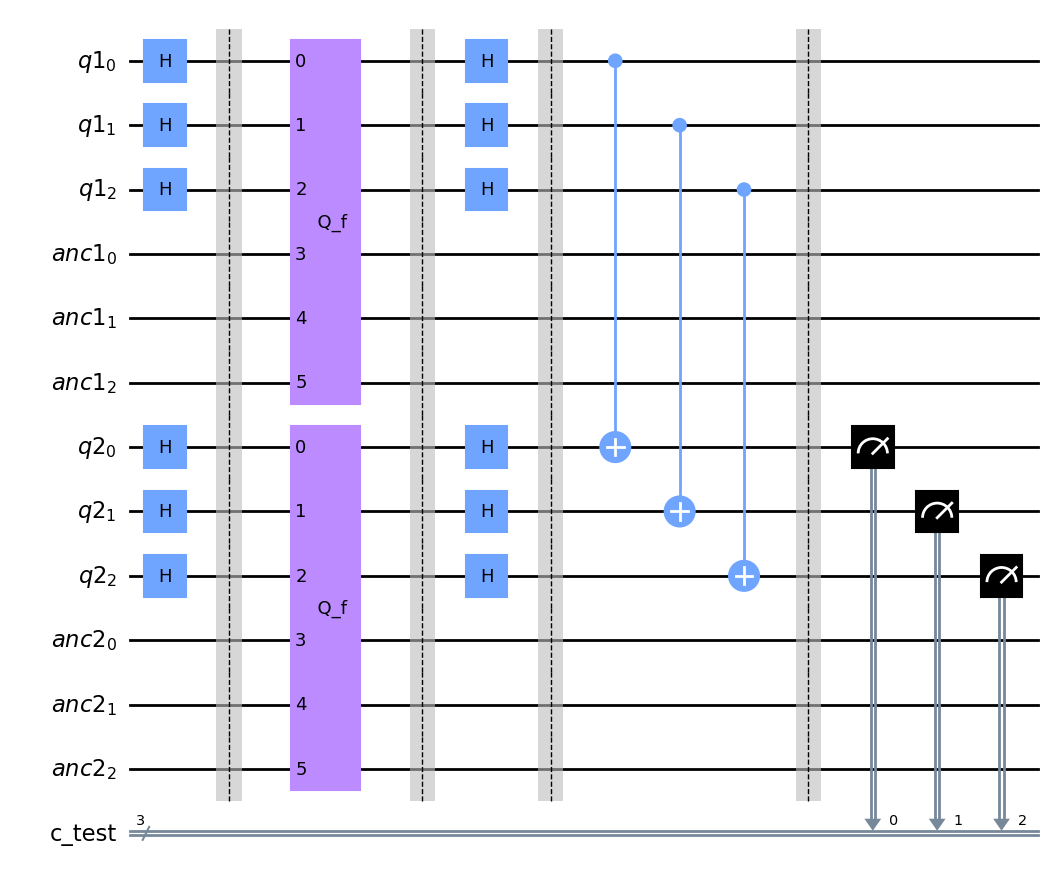
\includegraphics[width=0.8\textwidth]{TFG/imagenes/simonregla.png}
    \caption{Circuito, algoritmo Simon para la regla I con $\mathbf{c}=|001\rangle$}
    \label{Fig:CircuitoSimonR1}
 \end{figure}

 
 \begin{figure}[H]
    \centering
    \begin{subfigure}[H]{0.48\textwidth}
        \centering
        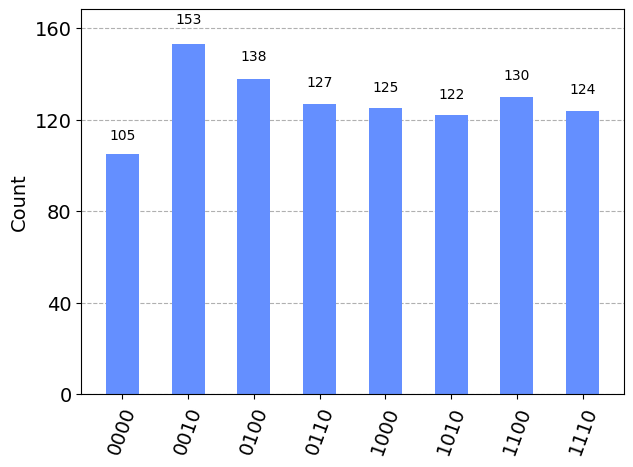
\includegraphics[width=\textwidth]{TFG/imagenes/resultadoSimon1.png}
        \caption{Algoritmo original}
        \label{sFig:Simon1.1}
    \end{subfigure}
    \hfill
    \begin{subfigure}[H]{0.48\textwidth}
        \centering
        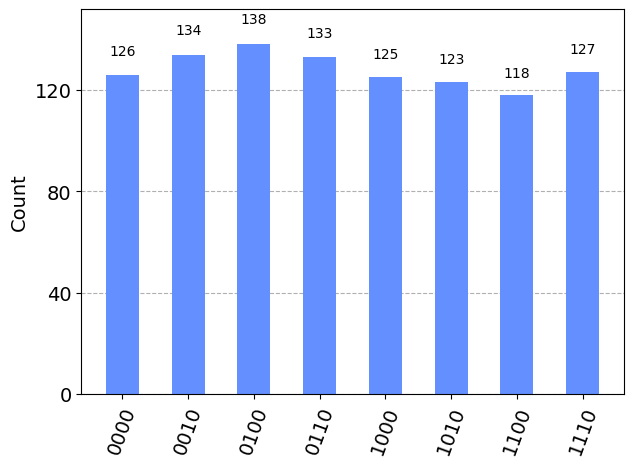
\includegraphics[width=\textwidth]{TFG/imagenes/resultadoRegla1Simon.png}
        \caption{Regla I}
        \label{sFig:Simon1.2}
    \end{subfigure}
        \caption{Resultados de la simulación del algoritmo Simon en el circuito original y en el circuito con la regla I implementada, para la cadena $\mathbf{c}=|0001\rangle$. }
    \label{FIG:Simon1.resultado}
 \end{figure}

\textbf{Regla II}: Si simulamos la implementación del algoritmo a una cadena $\mathbf{c}$ y se invierten las cadenas $\mathbf{z}\in S_{\mathbf{c}}$, equivale a aplicar el programa a $\mathbf{c}$ invertida.\newline

Esto se debe a que si permutamos los bits para realizar la inversión tanto en el \textit{source input} como en el \textit{output}, no estamos variando el resultado. Se entiende de manera más sencilla de manera matemática. Sean $M$ la matriz que realiza la inversión, no hay que olvidar que $M=M^{-1}$ y $\mathbf{z} \in S_{\mathbf{c}}$:

\begin{equation}
    \begin{split}
    \langle \mathbf{z},\mathbf{c} \rangle &= z_{1}c_{1} \oplus z_{2}c_{2} \oplus ...  \oplus z_{n}c_{n} \\ &= z_{n}c_{n} \oplus ... \oplus z_{2}c_{2} \oplus z_{1}c_{1} \\ &= \langle M\mathbf{z}, M\mathbf{c} \rangle = 0 \Rightarrow M\mathbf{z} \in S_{M\mathbf{c}}
    \end{split}
\end{equation}\newline

Esto se puede realizar de esta manera directa debido a que $\oplus$ es un operador conmutativo, por lo que incluso podríamos ampliar a que $(S_{\mathbf{c}},\oplus)$ es un grupo abeliano. Esto probaría la validez matemática de esta MR para el algoritmo de Simon. \newline

\textbf{Implementación}: simulamos el \hyperref[Fig:CircuitoSimon1]{algoritmo original} sobre $\mathbf{c}$ y $M\mathbf{c}$, invirtiendo una de las listas de cadenas obtenidas para comparar resultados. Estos pueden ser representados directamente en forma de listas, tal y como está en el documento o con la representación en histograma tras hacer la modificación.\newline

Todas estas simulaciones, así como el código para ambas reglas se pueden encontrar en el \href{https://github.com/rodelanu/TFG/tree/main}{repositorio común}, específicamente en el archivo sobre las \href{https://github.com/rodelanu/TFG/blob/main/3_Simon_Rules.ipynb}{reglas del algoritmo de Simon}.